\section*{Schutz der Nutzerdaten}
Da das System personenbezogene Informationen wie Nutzerdaten und Buchungsdetails 
verarbeitet, wurden verschiedene Sicherheitsmaßnahmen implementiert, um unbefugten 
Zugriff zu verhindern, die Datenintegrität zu gewährleisten und den 
Datenschutzbestimmungen zu entsprechen.
Eine wichtige Rolle spielt das Session-Handling. Nach einer erfolgreichen Anmeldung 
bleibt der Nutzer über eine Sitzung authentifiziert, sodass er nicht bei jeder Aktion 
erneut seine Zugangsdaten eingeben muss. Um die Sicherheit zu erhöhen, wird die Sitzung 
nach einer Inaktivitätszeit von 2 Minuten automatisch beendet. Dies schützt vor 
Missbrauch durch offene Sitzungen auf unbeaufsichtigten Geräten.
Zusätzlich wird bei einer abgelaufenen Sitzung ein Overlay angezeigt, das den Nutzer zur 
erneuten Anmeldung auffordert. 
\begin{center}
  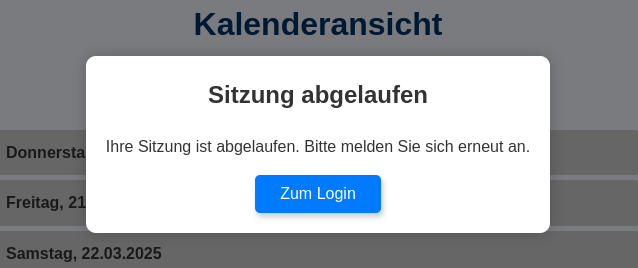
\includegraphics[width=0.95\linewidth, height=0.45\textheight, keepaspectratio]{src/abbildungen/session.png}
  \captionof{figure}{Sitzung abgelaufen}
\end{center}
Die Sitzungsinformationen werden ausschließlich 
serverseitig verwaltet und nicht im Browser gespeichert, um die Gefahr des 
Sitzungsdiebstahls zu minimieren. Um sicherzustellen, dass die Sitzungs-Cookies gegen 
Angriffe geschützt sind, wurden bestimmte Attribute gesetzt.
\vspace{0.5cm}
\begin{lstlisting}[language=java, caption={Cookie-Attribute}, captionpos=b]
 session.setMaxInactiveInterval(120);
 Cookie sessionCookie = new Cookie("JSESSIONID", session.getId());
 sessionCookie.setHttpOnly(true);
 sessionCookie.setSecure(true); 
 sessionCookie.setAttribute("SameSite", "Strict"); 
 response.addCookie(sessionCookie);
\end{lstlisting}
Sollte sich ein Nutzer ausloggen oder eine Sitzung ablaufen, wird die Session sofort 
ungültig gemacht, um Missbrauch durch Dritte zu verhindern.
Ein weiterer Aspekt ist die sichere Speicherung von Passwörtern. Um Nutzerkonten vor 
Brute-Force-Angriffen und kompromittierten Datenbanken zu schützen, werden Passwörter mit 
dem Algorithmus PBKDF2 gehasht. Dieser nutzt eine hohe Anzahl von Iterationen und einen 
zufälligen Salt-Wert, um den Rechenaufwand für Angreifer zu steigern.Dadurch wird 
verhindert, dass vorberechnete Hash-Tabellen (Rainbow Tables) verwendet werden können.
Ebenfalls wichtig zu erwähnen ist die Verwendung von QR-Codes zur Terminverifizierung. 
Nach einer erfolgreichen Terminbuchung erhalten Nutzer eine Buchungsbestätigung per Mail 
als PDF mit einem QR-Code, der bei der Ankunft im Impfzentrum gescannt wird. Um den 
Datenschutz zu gewährleisten, enthält der QR-Code jedoch keine sensiblen Informationen, 
sondern lediglich eine Buchungs-ID, die beim Scannen mit der Datenbank abgeglichen wird. 
Selbst wenn ein QR-Code in falsche Hände gerät, können daraus keine Rückschlüsse auf die 
Identität des Nutzers gezogen werden. Diese Maßnahme entspricht den Bestimmungen der 
DSGVO und stärkt das Vertrauen der Nutzer in die Anwendung.
